\section{Charaterization}

    %%%%%%%%%%%%%%%%%%%%%%%%%%%%%%%%%%%%%
	%%  Slide 1: <Scurve> %%
	%%%%%%%%%%%%%%%%%%%%%%%%%%%%%%%%%%%%%
    \begin{frame}
        \frametitle{Threshold and noise}
        Injection circuit: at the FE input a charge.
        Charge injected depends on the C$_{inj}$, different for each pixel
        \begin{multicols}{2}
            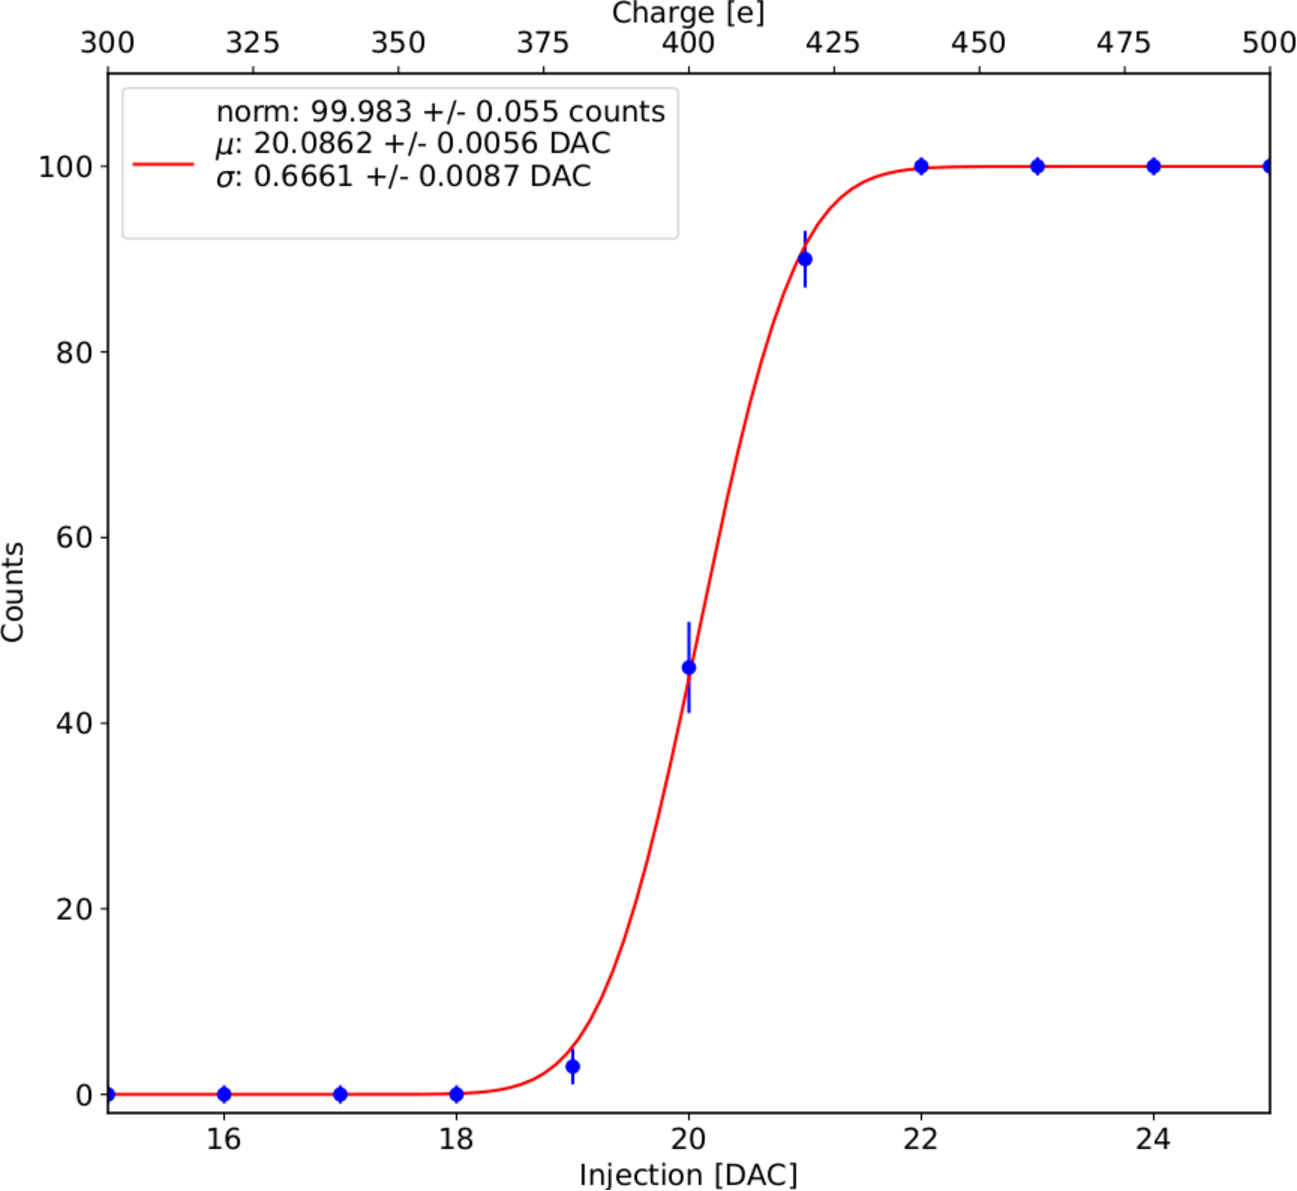
\includegraphics[width=1.\linewidth]{figures/charaterization/scurve.pdf}
        \columnbreak
            \begin{equation}
                erf=
            \end{equation}	
            Assuming a gaussian noise:\\
            threshold=$\mu$ \\
            noise=1/s=$\sigma$
        \end{multicols} 
 
    \end{frame}


    %\begin{center}
    %\end{center}
    
    %%%%%%%%%%%%%%%%%%%%%%%%%%%%%%%%%%%%%%%%
    %%  Slide 2: <Threshold_noise>  %%
    %%%%%%%%%%%%%%%%%%%%%%%%%%%%%%%%%%%%%%%%
    \begin{frame}
        \frametitle{Threshold and noise}
        \begin{figure}[h!]
            \centering
            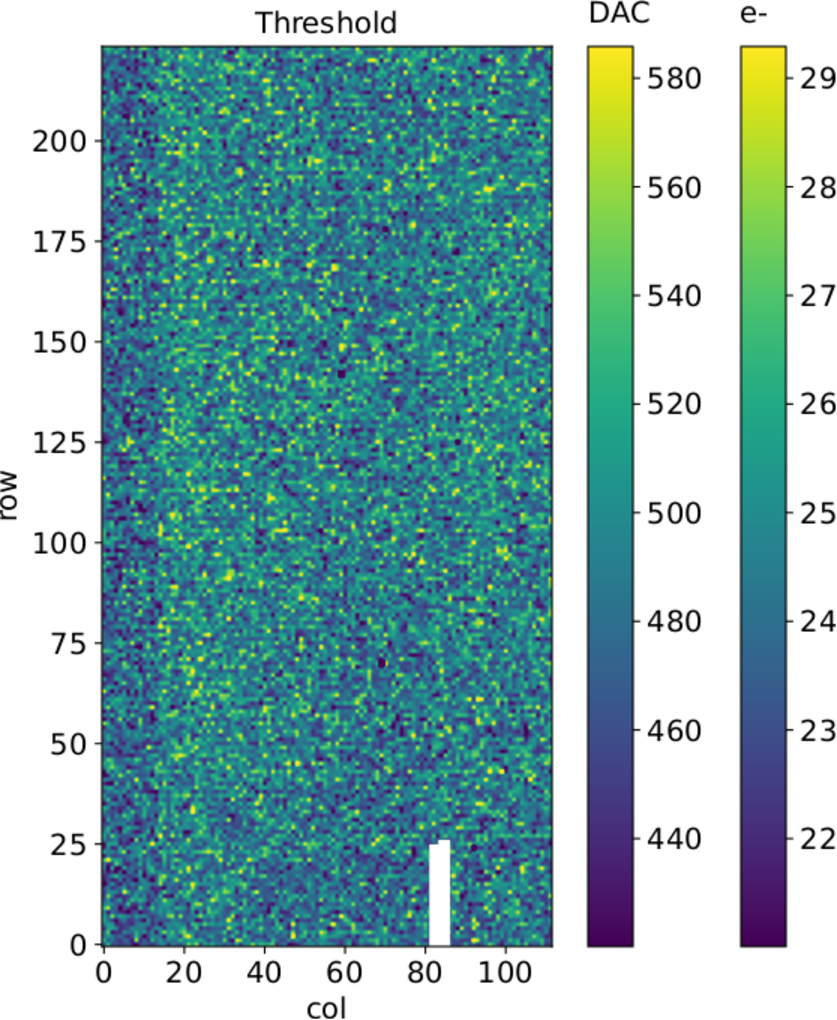
\includegraphics[width=.45\linewidth]{figures/charaterization/threshold_map.pdf}
            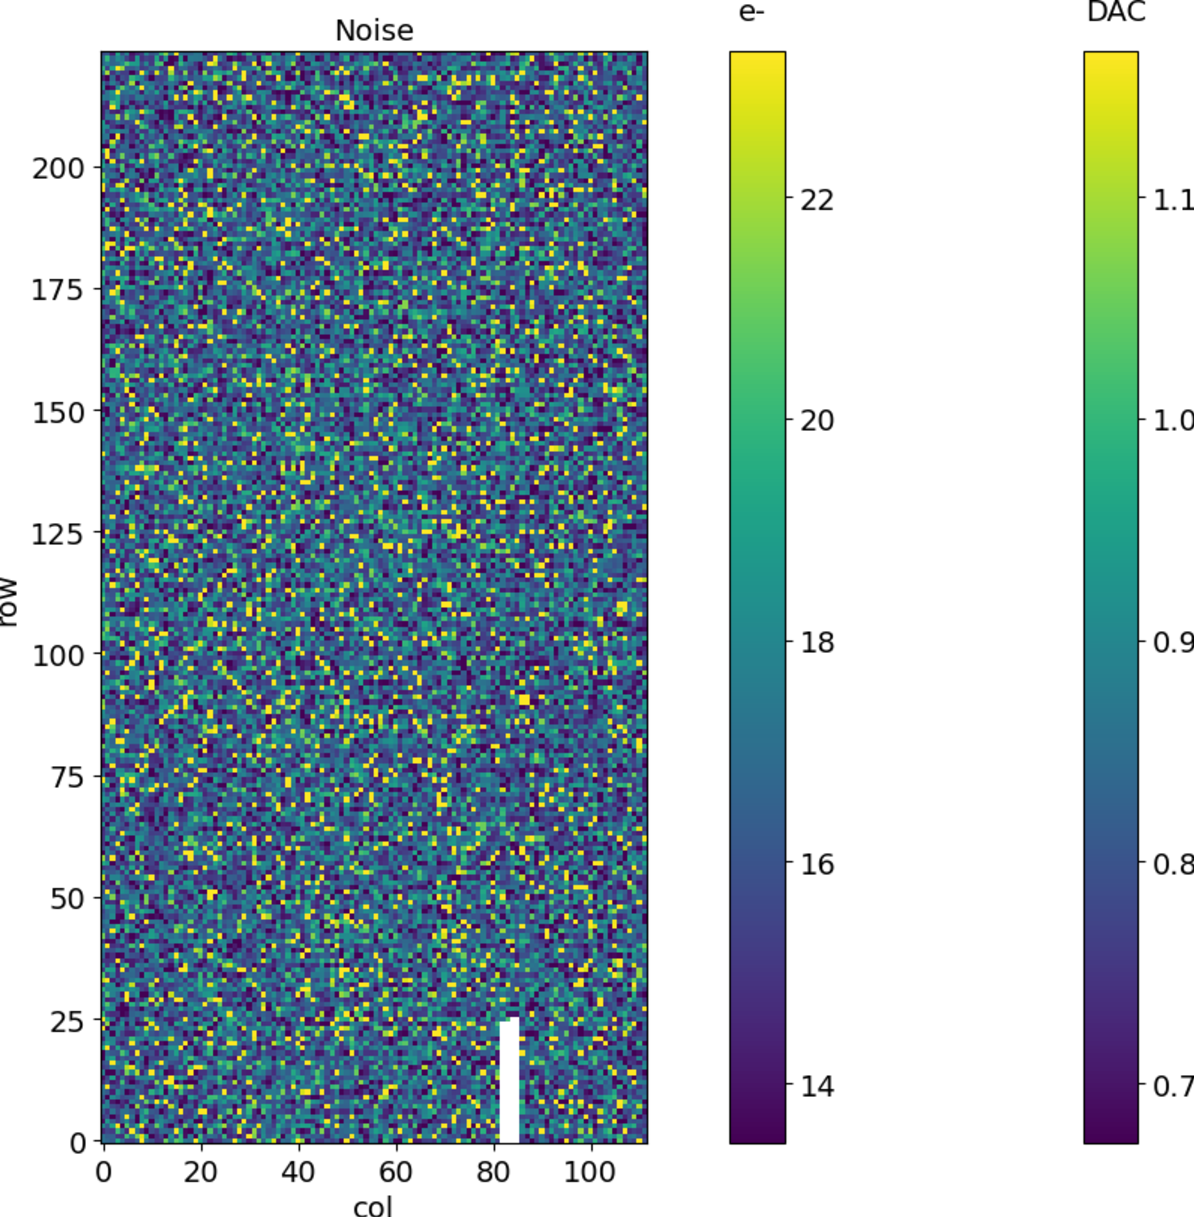
\includegraphics[width=.45\linewidth]{figures/charaterization/noise_map.pdf}
        \end{figure}
        Injection circuit broken
    \end{frame}

    %%%%%%%%%%%%%%%%%%%%%%%%%%%%%%%%%%%%%%%%
    %%  Slide 3: <ToT linearity>  %%
    %%%%%%%%%%%%%%%%%%%%%%%%%%%%%%%%%%%%%%%%
    \begin{frame}
        \frametitle{ToT linearity}
        \begin{itemize}
            \item The ToT linearity is due to the \textbf{PMOS} reset circuit which guaranties the costant discharge in time of the preamplifier (in general is not true)
            \item ToT is saved as a 6-bit variable
        \end{itemize}
        \medskip
        \medskip
        \medskip
        \begin{columns}
            \column{0.6\textwidth}  
                \centering
                Linearity tested with the injection
                \begin{figure}[h!]
                    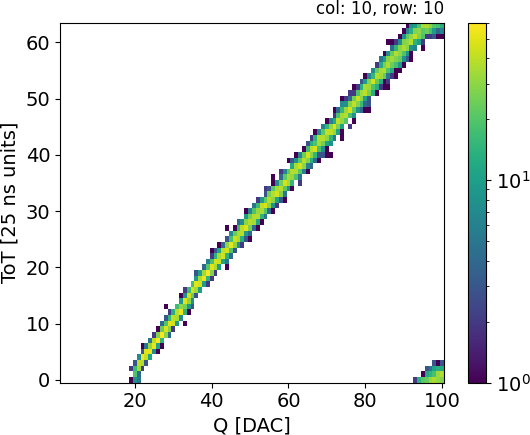
\includegraphics[width=.49\linewidth]{figures/charaterization/ToT_rollover.png}
                    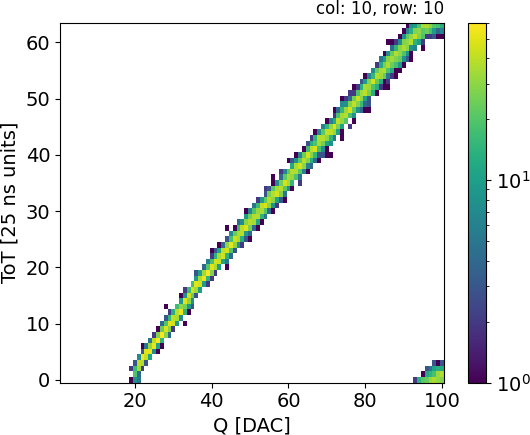
\includegraphics[width=.49\linewidth]{figures/charaterization/ToT_rollover.png} 
                \end{figure}
            \column{0.4\textwidth}
                \textbf{Rollover!}\\
                ToT varies in range 0-63

        \end{columns}
    \end{frame}    

    %%%%%%%%%%%%%%%%%%%%%%%%%%%%%%%%%%%%%%%%
    %%  Slide 4: <ToT vs charge>  %%
    %%%%%%%%%%%%%%%%%%%%%%%%%%%%%%%%%%%%%%%%
    \begin{frame}
        \frametitle{ToT vs charge }
        \begin{beamercolorbox}[sep=0em,wd=0.85\textwidth,ht=1.5ex, dp=0.1ex, rounded=true, center]{lightbluebox}
            Fe$^{55}$ $\rightarrow$ Mn$^{55}$ + K$_\alpha$ (\SI{5.9}{keV}) or K$_\beta$ (\SI{6.5}{keV})
        \end{beamercolorbox}

        \begin{tikzpicture}[overlay]
            \draw[decorate,decoration={brace}]
                (3.5,0) -- (5.5,0);
        \end{tikzpicture}


        with K$_\alpha$:
        \begin{itemize}
            \item $\lambda$=\SI{29}{\um}$\rightarrow$ P$_{abs}$=
            \item $w_i$=\SI{3.6}{eV} in Si @ \SI{300}{\kelvin}$\rightarrow$ \SI{1616}{\elementarycharge}$^-$
        \end{itemize}

        Provide a way 1) to measure the C$_{inj}$ and 2) calibrate the signal

    \end{frame}        

    %%%%%%%%%%%%%%%%%%%%%%%%%%%%%%%%%%%%%%%%
    %%  Slide 4: <ToT calibration>  %%
    %%%%%%%%%%%%%%%%%%%%%%%%%%%%%%%%%%%%%%%%
    \begin{frame}
        \frametitle{ToT calibration}
            \begin{figure}[h!]
                \centering
                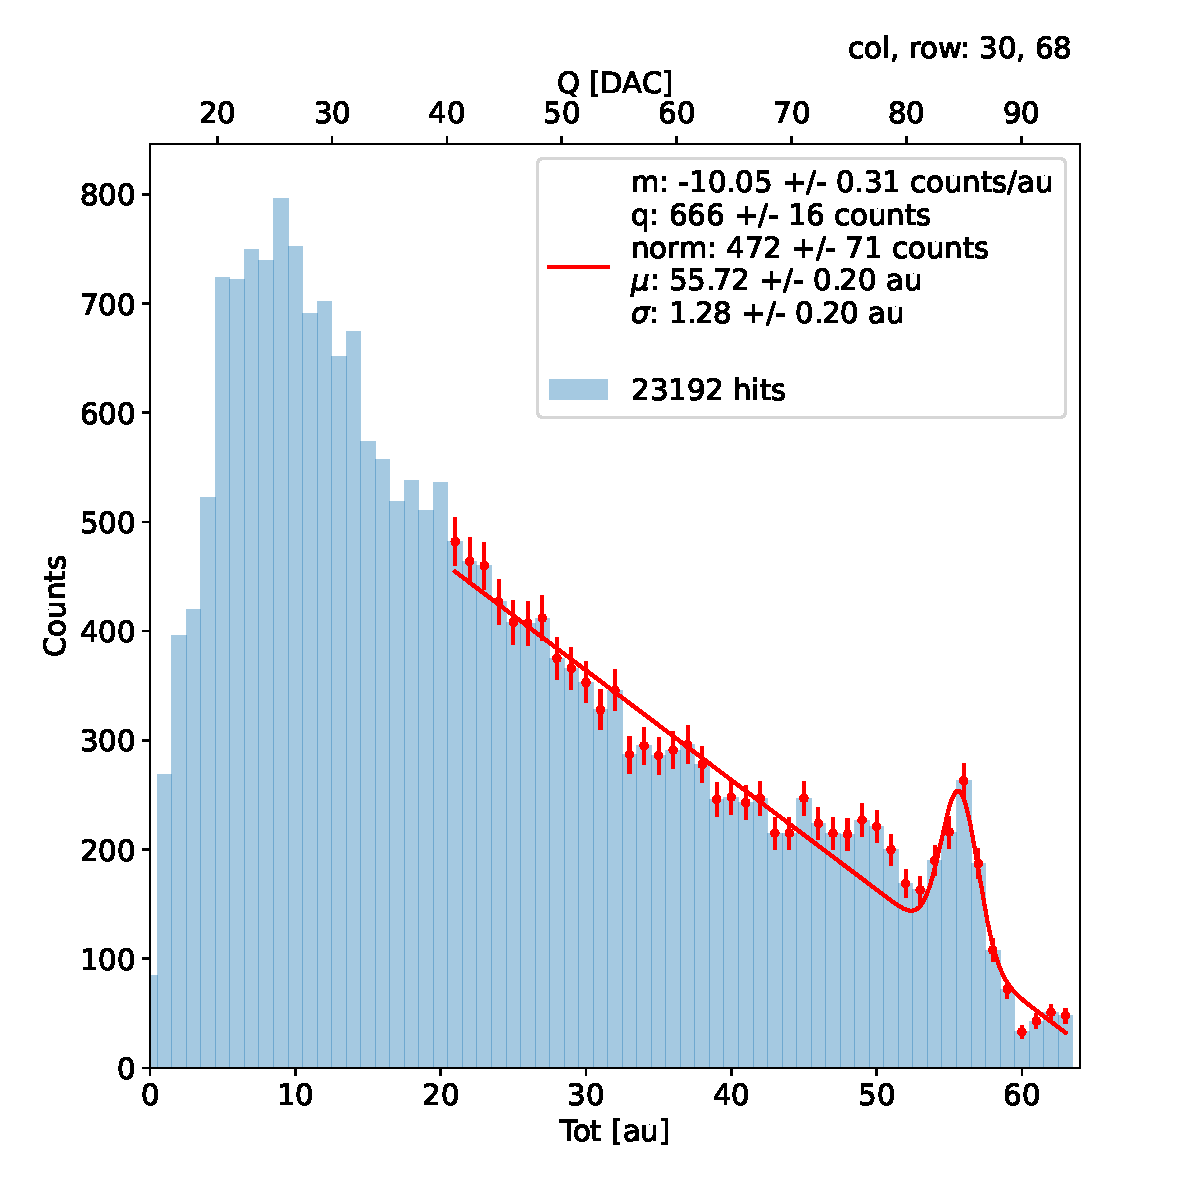
\includegraphics[width=.99\linewidth]{figures/charaterization/fit_line_gauss_r69.pdf}
            \end{figure}

    \end{frame}     


    %%%%%%%%%%%%%%%%%%%%%%%%%%%%%%%%%%%%%%%%
    %%  Slide 5: <ToT bias>  %%
    %%%%%%%%%%%%%%%%%%%%%%%%%%%%%%%%%%%%%%%%
    \begin{frame}
        \frametitle{Bias}
        \begin{figure}[h!]
            \centering
            %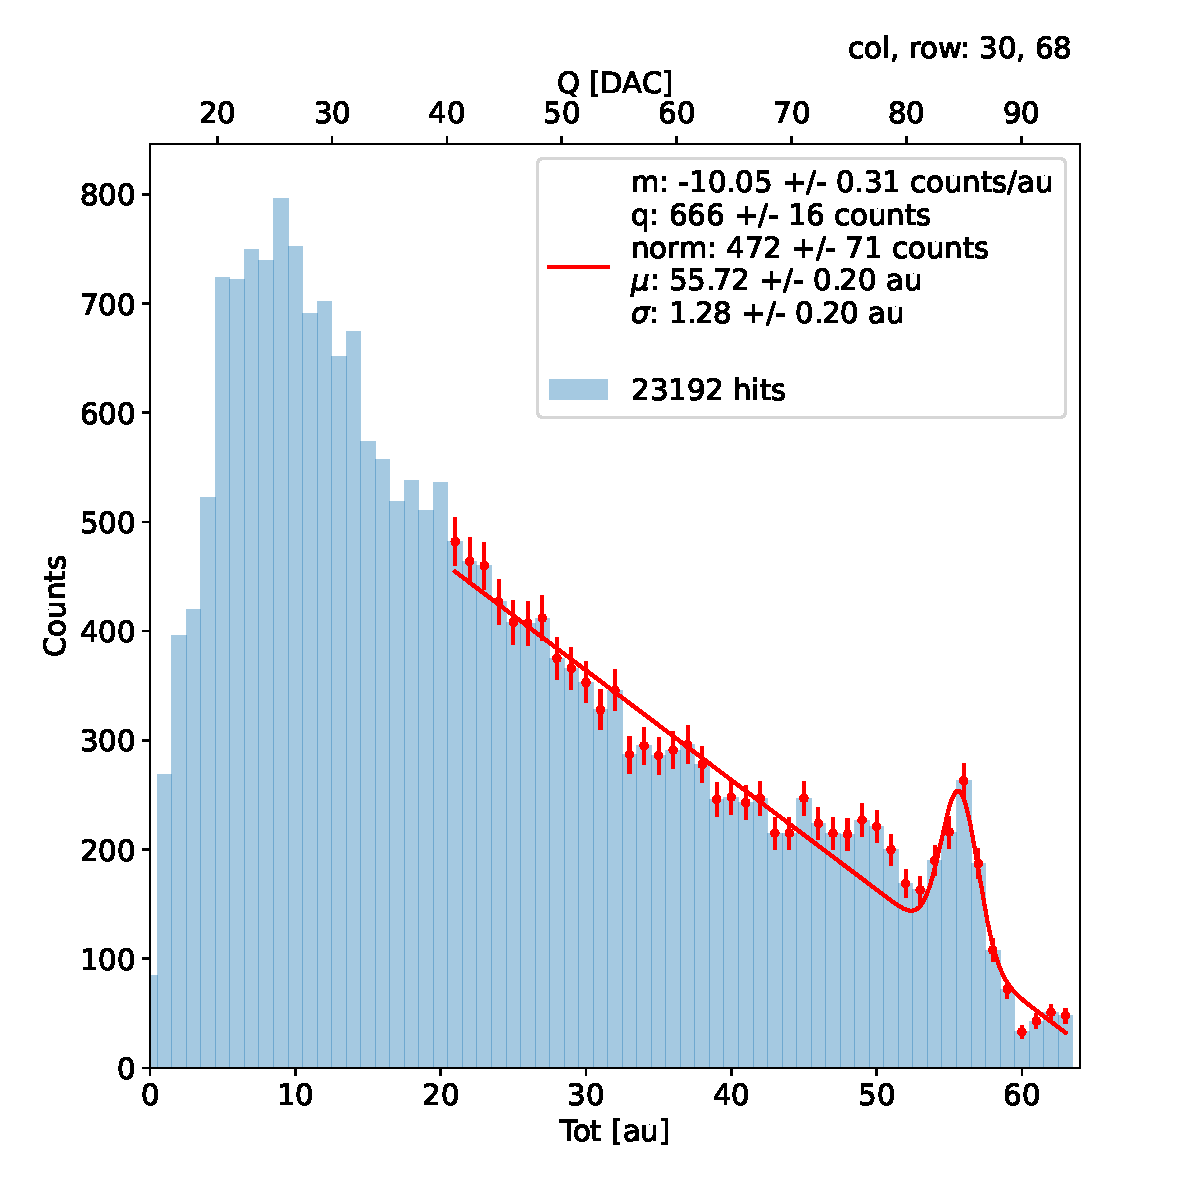
\includegraphics[width=.2\linewidth]{figures/charaterization/fit_line_gauss_r69.pdf}
        \end{figure}
    \end{frame}      

    %%%%%%%%%%%%%%%%%%%%%%%%%%%%%%%%%%%%%%%%
    %%  Slide 5: <Dead time>  %%
    %%%%%%%%%%%%%%%%%%%%%%%%%%%%%%%%%%%%%%%%
    \begin{frame}
        \frametitle{Readout time}
        \begin{figure}[h!]
            \centering
            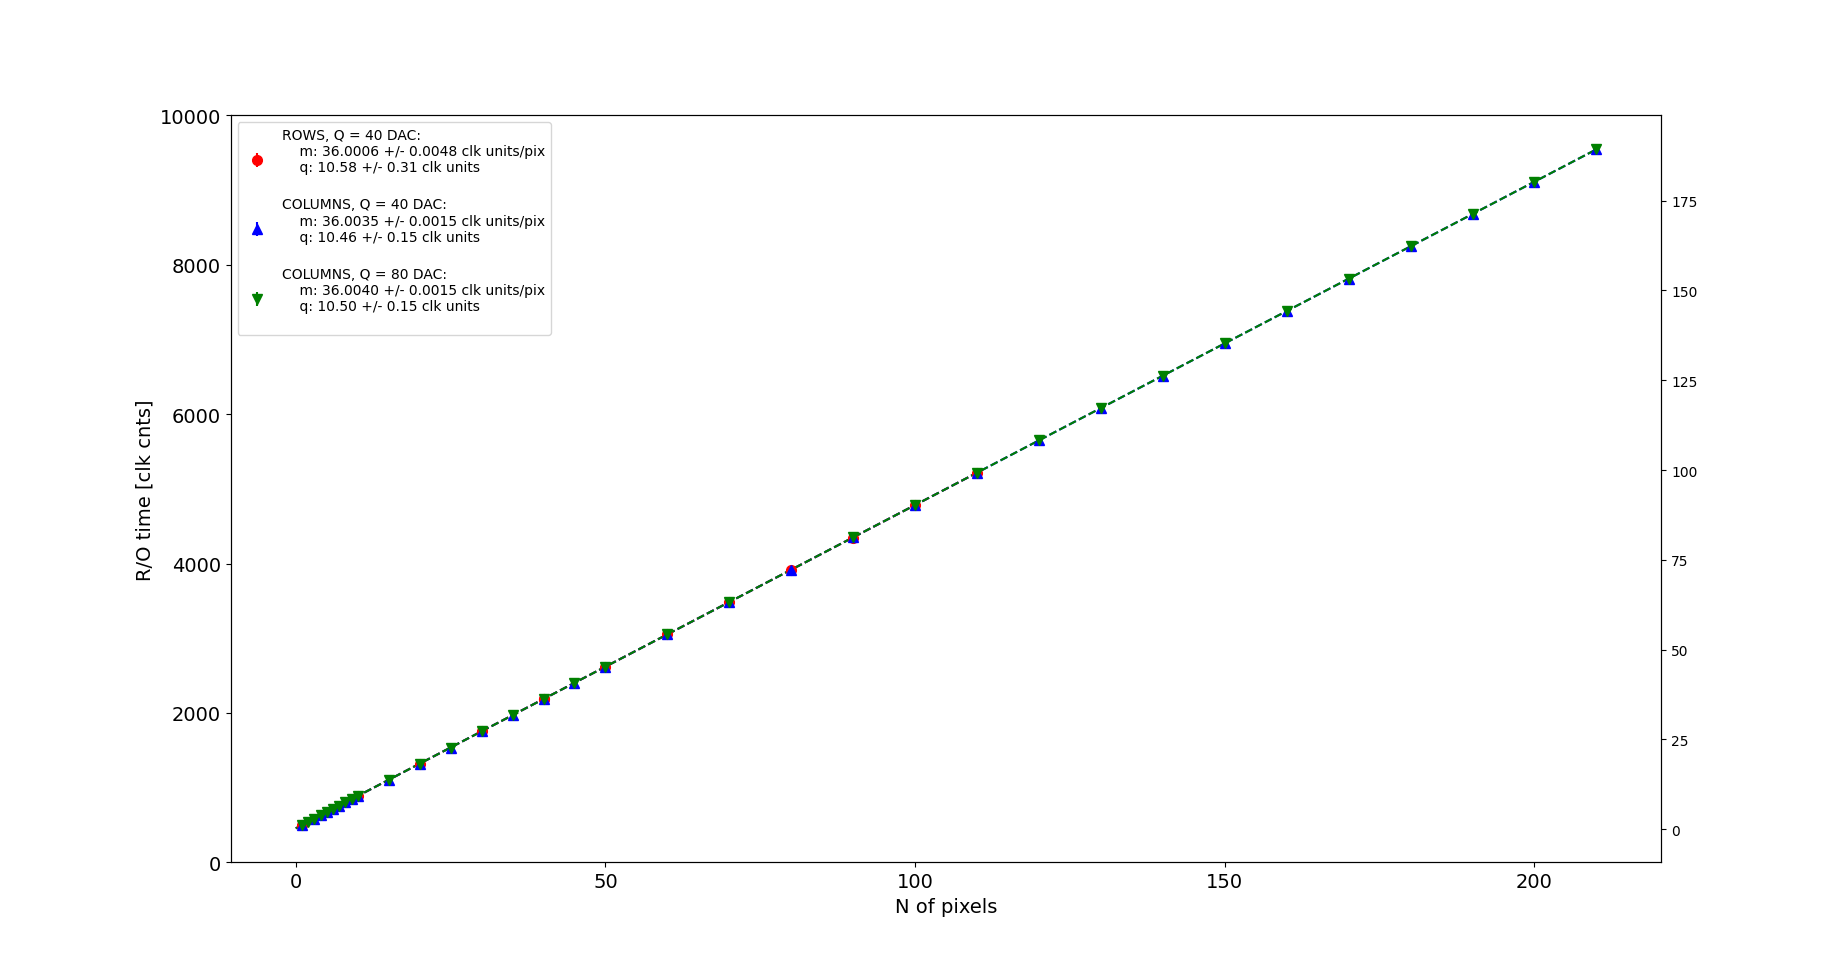
\includegraphics[width=.2\linewidth]{figures/charaterization/default_line.png}
        \end{figure}
    \end{frame}          